\documentclass{article}

% Symbols
\usepackage{amsfonts, amsthm}
\usepackage{upgreek}
\usepackage{physics}
\usepackage{cancel}
\usepackage{amssymb, latexsym, amsmath}
\usepackage{ stmaryrd }

%Algorithms
\usepackage[ruled,lined,linesnumbered,commentsnumbered]{algorithm2e}

%% Identación
\setlength{\parindent}{0cm}

% Comentario en bloques:
\iffalse
\fi

% Hipervínculos:
\usepackage{hyperref}

% Código
\newcommand{\code}[1]{\textcolor{white!25!black}{\texttt{#1}}}
\usepackage{listings}

%AMS
\usepackage{amsthm}
\newtheorem{algo-thm}{Algoritmo}

% Proof
\renewcommand*{\proofname}{\textbf{Demostraci\'on:}}
% Theorem
\newtheorem*{theorem}{Teorema}

% Graphics
\usepackage{graphicx}
\usepackage{pgf}

% Color a letras.
%\usepackage[usenames,dvipsnames,svgnames,table]{xcolor}

% Tikz
\usepackage{tkz-graph}
\usepackage{tikz}
\usetikzlibrary{arrows,automata}
\usepackage{tikz}
\usetikzlibrary{arrows,automata}
%\usetikzlibrary[topaths]
\usetikzlibrary{angles, quotes}
\usepackage{siunitx}

% Def. Dr. César.
\usetikzlibrary{shapes,calc}
\tikzstyle{edge}=[shorten <=2pt, shorten >=2pt, >=stealth, line width=1.1pt]
\tikzstyle{edgeDotted}=[shorten <=2pt, shorten >=2pt, >=stealth, line width=1.1pt, dashed] %  dashed
\tikzstyle{edgeC}=[curve to, out=270,in=270,relative, dashed]
\tikzstyle{blueE}=[shorten <=2pt, shorten >=2pt, >=stealth, line width=1.5pt, blue]
\tikzstyle{redE}=[shorten <=2pt, shorten >=2pt, >=stealth, line width=1.5pt, red]
\tikzstyle{blackV}=[circle, fill=black, minimum size=6pt, inner sep=0pt, outer sep=0pt]
\tikzstyle{brownV}=[circle, fill=brown, draw, minimum size=6pt, line width=0.75pt, inner sep=0pt, outer sep=0pt]
\tikzstyle{blueV}=[circle, fill=blue, draw, minimum size=6pt, line width=0.75pt, inner sep=0pt, outer sep=0pt]
\tikzstyle{redV}=[circle, fill=red, draw, minimum size=6pt, line width=0.75pt, inner sep=0pt, outer sep=0pt]
\tikzstyle{redSV}=[semicircle, fill=red, minimum size=3pt, inner sep=0pt, outer sep=0pt, rotate=225]
\tikzstyle{blueSV}=[semicircle, fill=blue, minimum size=3pt, inner sep=0pt, outer sep=0pt, rotate=225]
\tikzstyle{blackSV}=[semicircle, fill=black, minimum size=3pt, inner sep=0pt, outer sep=0pt, rotate=225]
\tikzstyle{vertex}=[circle, draw, minimum size=6pt, line width=0.75pt, inner sep=0pt, outer sep=0pt]

%%%%%%%%%%%%%%%%%%%%%%%%%%%%%%%%%%%%%%%%%%%%%%%%%%%%%%%%%
\newcommand\Star[3][]{%
\path[#1] (0  :#3) -- ( 36:#2) 
       -- (72 :#3) -- (108:#2)
       -- (144:#3) -- (180:#2)
       -- (216:#3) -- (252:#2)
       -- (288:#3) -- (324:#2)--cycle;}
%%%%%%%%%%%%%%%%%%%%%%%%%%%%%%%%%%%%%%%%%%%%%%%%%%%%%%%%%
% Margins
\addtolength{\voffset}{-1.5cm}
\addtolength{\hoffset}{-1.5cm}
\addtolength{\textwidth}{3cm}
\addtolength{\textheight}{3cm}

% Columnas multiples
\usepackage{multicol}

%Header-Footer
\usepackage{fancyhdr}
\renewcommand{\headrulewidth}{1pt}

\newcommand{\set}[1]{
  \left\{ #1 \right\}
}

%\pagenumbering{gobble} -- Este comando
%                       -- quita el número de página.
\footskip = 50pt
\renewcommand{\headrulewidth}{1pt}

\pagestyle{fancyplain}

\begin{document}
\title{UNIVERSIDAD NACIONAL AUT\'ONOMA DE M\'EXICO\\ Facultad de Ciencias}
\author{Autor: Adri\'an Aguilera Moreno}
\date{}
\maketitle
\begin{center}
  
\includegraphics[scale=0.20]{../Imagen/Portada.jpg}\\[0.4cm]
  \Large
  \bf{Algoritmos II}
  \normalsize
\end{center}
\newpage
\fancyhead[r]{ Algoritmos II.}
%%%%%%%%%%%%%%%%%%%%%%%%%%%%%%%%%%%%%%%%%%%%%%%%%%%%%
\section*{\LARGE{Resumenes.}}
%%%%%%%%%%% Exposición 01
\subsection[Expositor: Adrián Aguilera.]{Un algoritmo de barrido de línea para agrupamiento espacial.}
\textbf{Obejetivo:} Agrupar un conjunto de puntos $P$ en el plano de manera
jerárquica, por medio de la distancia que los separa entre sí. \newline

\textbf{Desarrollo:} El algoritmo consiste en, dadas dos líneas
$s_1$ y $s_2$, y $P$ ordenado. Entonces barremos $P$ con ambas
líneas y dejando una separación $d$ entre $s_1$ y $s_2$. \newline

En la primer iteración, agrupamos los puntos a una cercanía $\frac{d}{2}$ y coloreamos
bajo un mismo color los puntos que han sido agrupados en un mismo punto. En esta iteración
creamos el FRENTE DE AVANCE (AF), que esta dado por la trayectoria entre los puntos
coloreados a este punto. \newline

En la $i$-ésima iteración,


\newpage
%%%%%%%%%%% Exposición 02
\subsection[Expositor: Raúl Nuño Valdés.]{Un algoritmo de barrido de línea y su aplicación en espirales interiores (pocketing).}
\textbf{Obejetivo:} Construcción de espirales internas a un polígono dado. \newline

\textbf{Desarrollo:} Una alternaiva mencionada es usar los diagramas de Voronoi. Sin embargo, la
estrategia seguida es:
\begin{enumerate}
\item Ordenar nuestro arreglo de puntos.
\item Crear nuestro polígono. \newline
  
  En este punto nos interesa encontrar polígonos válidos, esto lo logramos búscando en
  el orden de las manecillas del reloj: empezamos en un punto y recorremos hasta toparnos
  con que no podemos avanzar y eliminamos esa arista (pues no será parte de nuestro polígono
  admisible).
\item Eliminar colineales.\newline

  No tiene sentido tener puntos colineales en el polígono, pues construiremos
  las espirales internas a partir de estos (todos) y solo nos interesa tener segmentos, sin importar si
  hay más de dos puntos en ellos.
\item Encontrar un extremo (caso partícular del extremo izquierdo).\newline
  
  Esto lo usamos para empezar el barrido y lo podemos encontrar en tiempo constante si ordenamos nuestro
  arreglo o en tiempo líneal en otro caso.
\item Barrido de línea. \newline
  
  Nos toma $\mathcal{O}(\log n)$ por punto, pues empezamos a contruir las espirales.
\item Encontrar intersecciones entre monótonas.\newline
  
  Las intersecciones serán parte de la construcción de la espiral.  
\item Obtener el arreglo de intersecciones. \newline
  
  Lo obtenemos del paso anterior en $\mathcal{O}(n \log n)$.
\end{enumerate}

\textbf{Obs.} El algoritmos consiste en ir acotando la súperficie interna del polígono e ir formando las espirales en estas
áreas. Debemos saber cuándo parar, esto es cuándo acotamos la sección llamada isla, en este punto el polígno debe tener
espirales internas y tener estas construcciones terminadas.\newline

\textit{Análisis de complejidad.} La complejidad esta contenida en
\[\therefore\: \mathcal{O}(n) + \mathcal{O}(n \log n) = \mathcal{O}(n \log n).\]

\newpage
%%%%%%%%%%% Exposición 03
\subsection[Expositor: Juan Manuel Díaz Quiñonez.]{Iluminación de polígonos con refelctores.}
\textbf{Obejetivo:} Cotas sobre el número de reflectores suficientes para iluminar un polígono simple.\newline

\textbf{Desarrollo:} Para cada vértice $p_i$ en el polígono se asignan pesos de $\alpha_i$ correspondiente
al ángulo de iluminación a partir de $p_i$. Cabe mencionar que no es cierto que para cada $p_i$ corresponda
un $\alpha_i$ necesariamente.\newline

Dado un subconjunto S de los vértices de P, decimos que $S$ ilumina a P si todo punto de P es visible desde algún
vértice en $S$. Asociaremos un peso a $S$ igual a la suma de los pesos de los elementos de $S$.

\begin{center}
  \textbf{Teo 1.} Todo polígono $P$ con $n$ vértices tiene un subconjunto $S$
  que lo ilumina de tal manera que el peso de $S$ es a lo más
  \[\frac{(n - 2)\pi}{3}.\]
  Para cada $\epsilon > 0$ existen polígonos tales que
  no tienen conjuntos de vértices que los iluminen de peso
  \[\frac{(n - 2)\pi}{3} - \epsilon.\]
\end{center}


\begin{center}
  \textbf{Teo 2.} Para cualquier $\epsilon > 0$, existen polígonos simples que no
  pueden ser iluminados con reflectores de tamaño menor o igual a $\pi - \epsilon$
  aún permitiendo un reflector por vértice. A nosotros nos importará demostrar que esto es cierto
  para $\epsilon \geq \frac{1}{2}$.
\end{center}

\begin{center}
  \textbf{Teo 3.} Todo polígono ortogonal sin agujeros puede iluminarse
  con a lo más
  \[\lfloor \frac{3n - 4}{8} \rfloor\]
  reflectores ortogonales.
  
  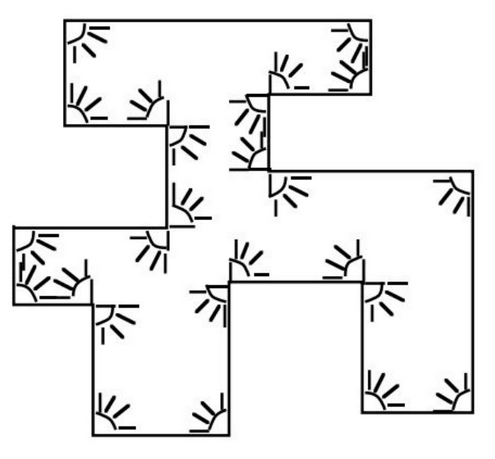
\includegraphics[scale=0.40]{./Im1.png}\\[0.4cm]
\end{center}

\begin{center}
  \textbf{Teo 4.} Todo polígono ortogonal $P$ con $h$ agujeros y $n$ vértices
  puede iluminarse con a lo más
  \[\lfloor\frac{3n + 4(h-1)}{8}\rfloor\]
  reflectores ortogonales colocadas sobre los vértices de $P$.
\end{center}

\begin{center}
  \textbf{Teo 5.} Todo polígono ortogonal $P$ con $n$ vértices puede
  iluminarse con a lo más
  \[\lfloor \frac{n}{4}\rfloor\]
  reflectores sobre la frontera de $P$.
  Dichos reflectores pueden ser localizados
  en tiempo lineal. Resultado mostrado en la exposición de \textit{Ares Castro Romero.}
\end{center}


\newpage
%%%%%%%%%%% Exposición 03
\subsection[Expositor: Zayra Paulina Galván Ordoñez.]{Un problema simple de caminos alternos.}
\textbf{Obejetivo:} Resolver el problema de Putman para una cadena círcular partícular y dar el conjunto de posibles caminos
en una gráfica que se pueden tomar para llegar a la palabra dada, en caso de ser admisible. Esto es, ¿de cuántas maneras
podemos formar la cadena siempre que sea admisible?.\newline

\textbf{Desarrollo:} Nos basamos en las reglas de construcción:
\begin{itemize}
\item La palabra vacía es válida.
\item $abW$, dónde $W$ es no terminal (en adelante se omite la explicación).
\item $aWb$.
\item $bWa$.
\item $Wab$.
\end{itemize}
ahora, debemos contar las posiciones en la palabra círcular $c$. Enumeremos carácter
a carácter con $s_i$ y cuán queramos acceder a un carácter $j > |c|$, entonces buscaremos
el carácter en la posición $j \mod c$. Utilizaremos la notación $W(i, j)$ tal que iniciaremos
en el carácter $i$ y elijiremos los siguientes $k \cdot j$ carácteres de manera círcular y donde
$k$ es el número de carácteres de la palabra por nivel de jerárquia. \newline

¿Qué son los niveles de jerárquia? Les llamo partícularmente a los niveles que se forman en nuestra
gráfica, iniciando con la vacía, luego con $W(i,1), W(i,2), \dotsm$\newline

Ya definidos los niveles, entonces tenemos como ``fuente'' a la palabra vacía y como ``sumidero'' a la
palabra círcular objetivo, así basta bajar desde la fuente al sumidero en forma de aristas orientadas
para saber cuántas maneras hay de formar la palabra. Las palabras relacionadas por una arista serán
aquellas que procedan por medio de una regla de producción (de las ya mencionadas). \newline

Si la palabra círcular es no-admisible, entonces no hay manera de llegar por un camino desde la fuente
al sumidero. \newline

\textit{Análisis de complejidad.} Basta ver que en el pero de los casos es necesario construir la gráfica
que por cada nodo inicial (donde nace la arista orientada) tenga relación con todos los nodos en el siguiente
nivel, en general esto es un orden cuadrático y por tanto la complejidad de nuestro algoritmo es $\mathcal{O}(n^2)$.

\newpage
%%%%%%%%%%% Exposición 03
\subsection[Expositor: Zayra Paulina Galván Ordoñez.]{Segmentos de líneas punzantes.}
\textbf{Obejetivo:} Algoritmo para determinar las líneas que interseca a cada uno de
los $n$ segmentos de línea dados en el plano.\newline

\textbf{Desarrollo:} Para un conjunto $S$ de $n$ segmentos de línea en el plano. Si queremos calcular
todas las líneas punzantes, entonces analicemos dos posibles casos:
\begin{enumerate}
\item Si sólo hay un segmento de línea en el conjunto $S$.
  Entonces, la región punzante es la doble cuña de este segmento.
  
  \begin{center}
    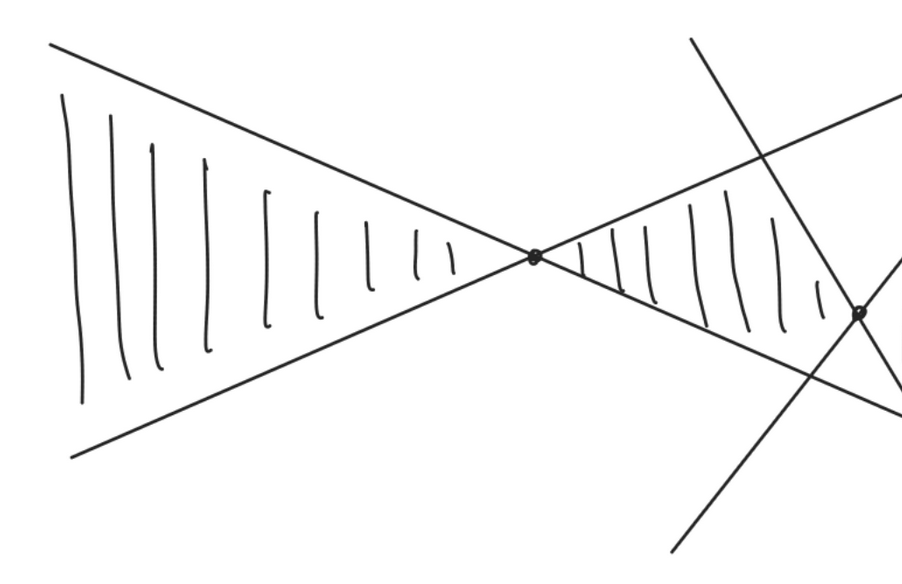
\includegraphics[scale=0.30]{./Im2.png}\\[0.4cm]
  \end{center}
\item Si hay al menos dos segmentos, dividir el conjunto $S$ en dos subconjuntos
  de igual tamaño y calcular la región punzante de ambos subconjuntos de manera
  recursiva. La región punzante de todo el conjunto es la intersección de las
  regiones punzantes de los subconjuntos.
\end{enumerate}

\end{document}
